\section*{Задание}

Используя хвостовую рекурсию, разработать программу, позволяющую найти
\begin{enumerate}
	\item n!,
	\item n-е число Фибоначчи.
\end{enumerate}

Убедиться в правильности результатов.

Для одного из вариантов ВОПРОСА и каждого задания составить таблицу,
отражающую конкретный порядок работы системы:

Т.к. резольвента хранится в виде стека, то состояние резольвенты требуется отображать
в столбик: вершина – сверху! Новый шаг надо начинать с нового состояния резольвенты!
\begin{lstinputlisting}[label=third,caption=Решение задания №1, language=prolog, firstline=1, lastline=22]{../src/lab_16.pro}
\end{lstinputlisting}
\begin{figure}[H]
	\caption{Таблица к заданию.}
	\begin{center}
		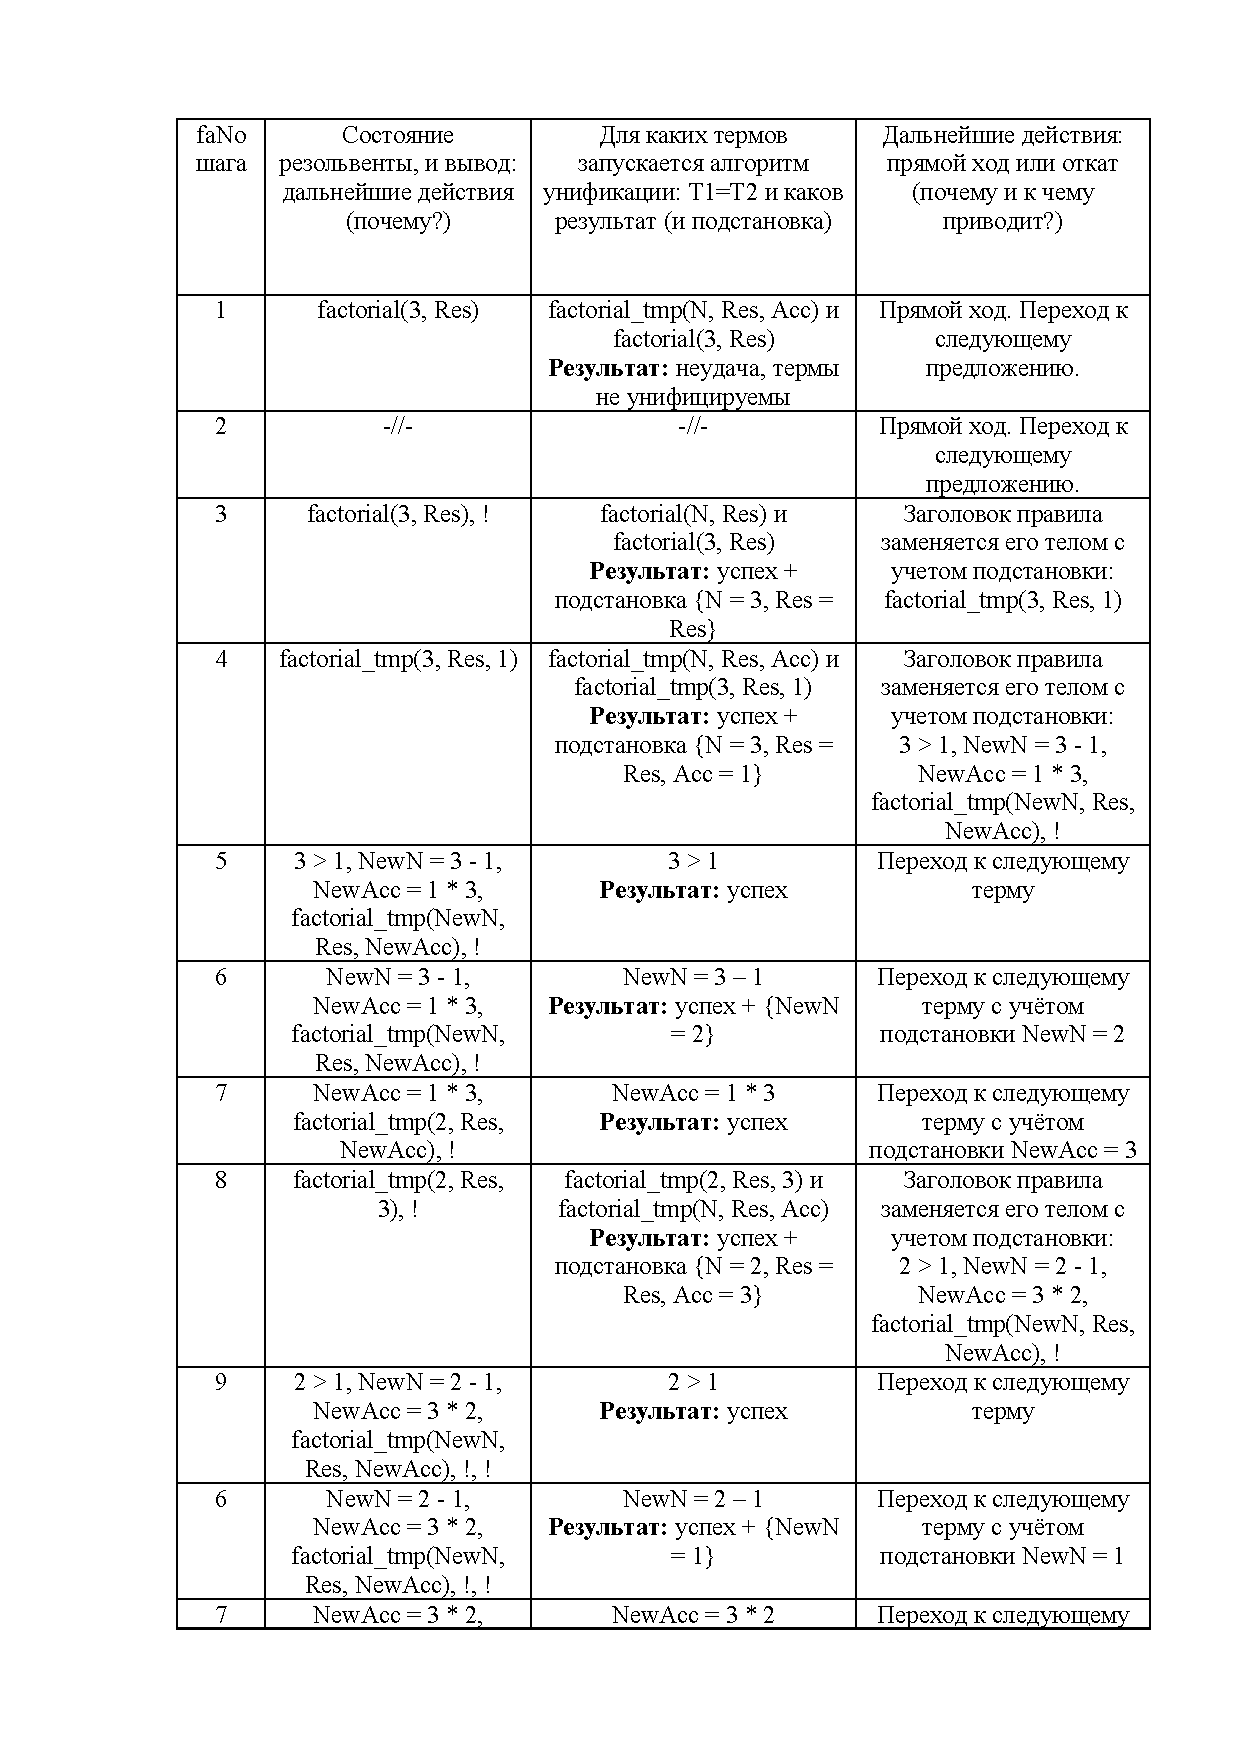
\includegraphics[scale=0.85]{img/16.1.pdf}
	\end{center}
	
\end{figure}

\begin{figure}[H]
	\begin{center}
		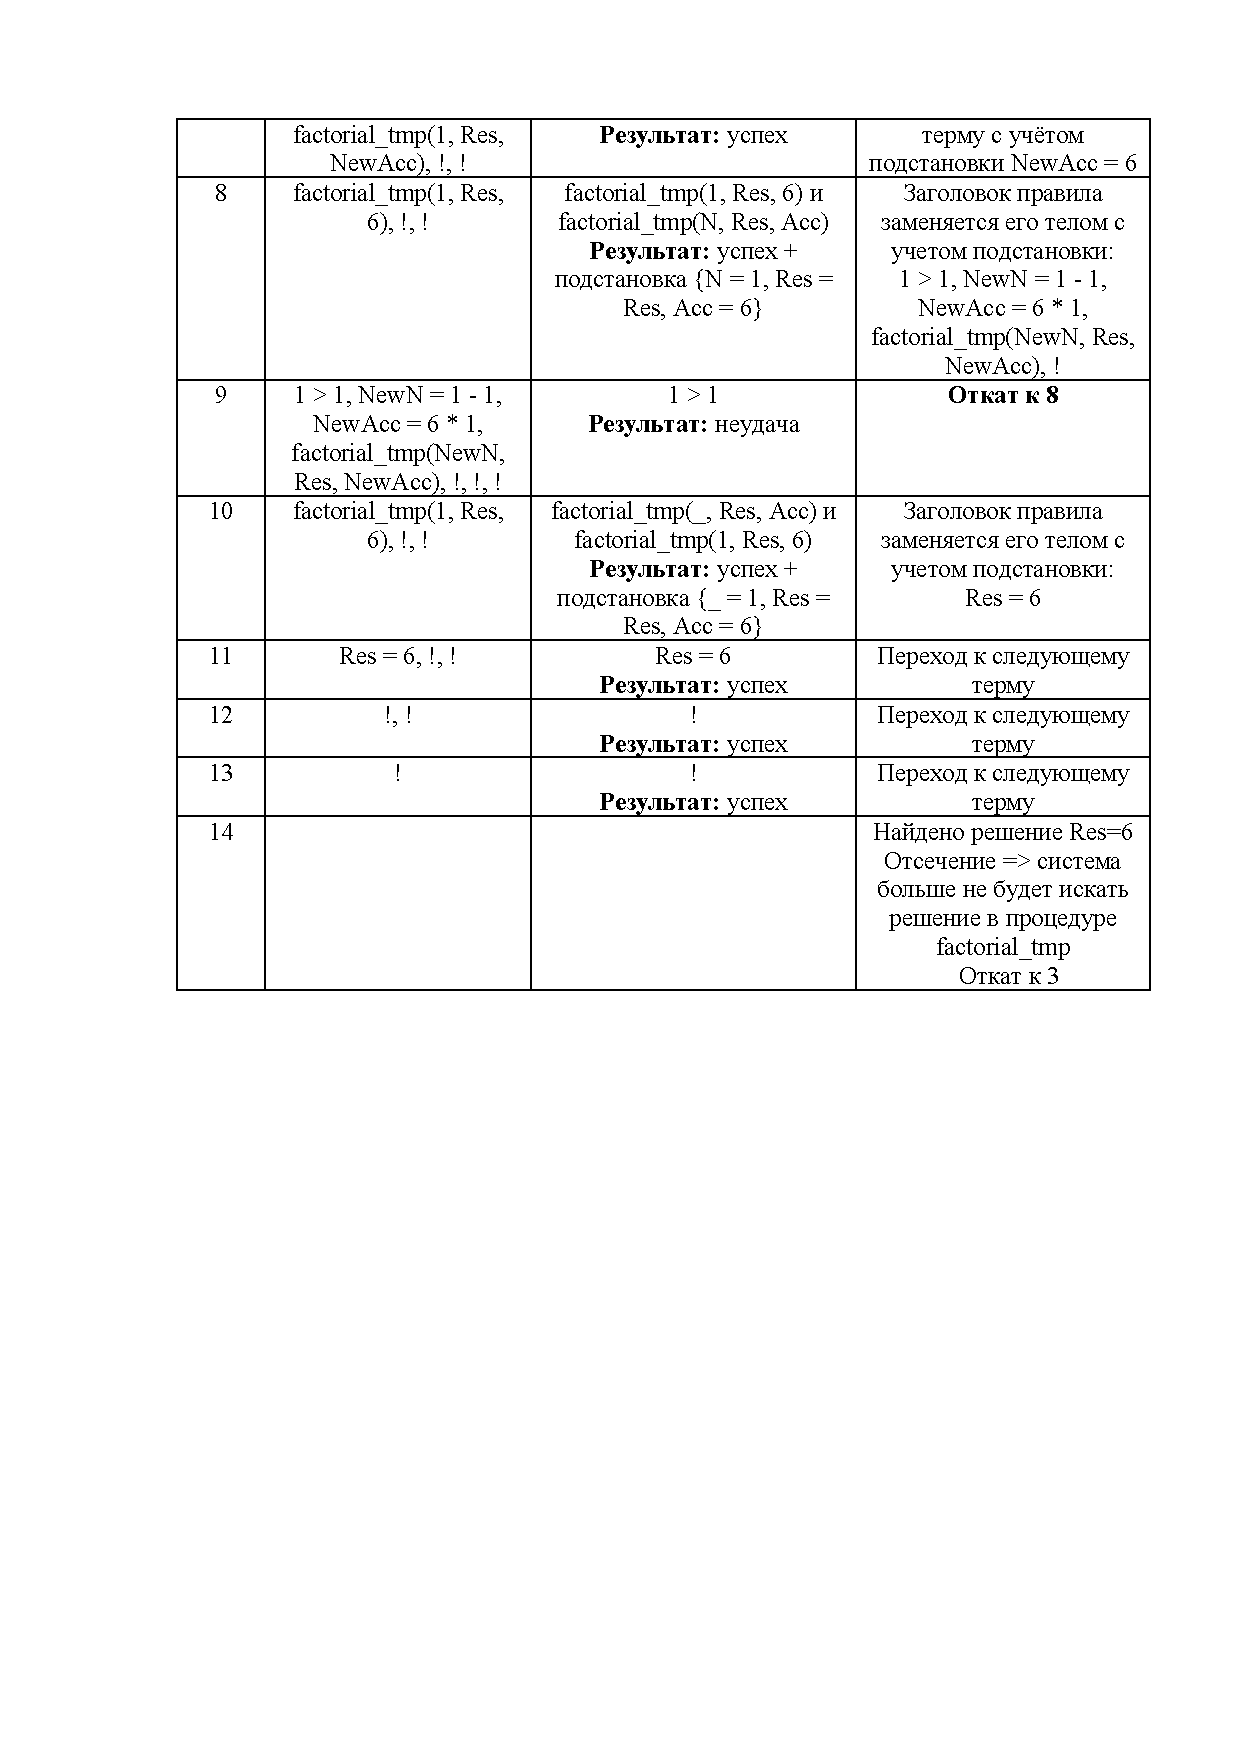
\includegraphics[scale=0.85]{img/16.2.pdf}
	\end{center}
\end{figure}